\begin{figure*}
    \centering
    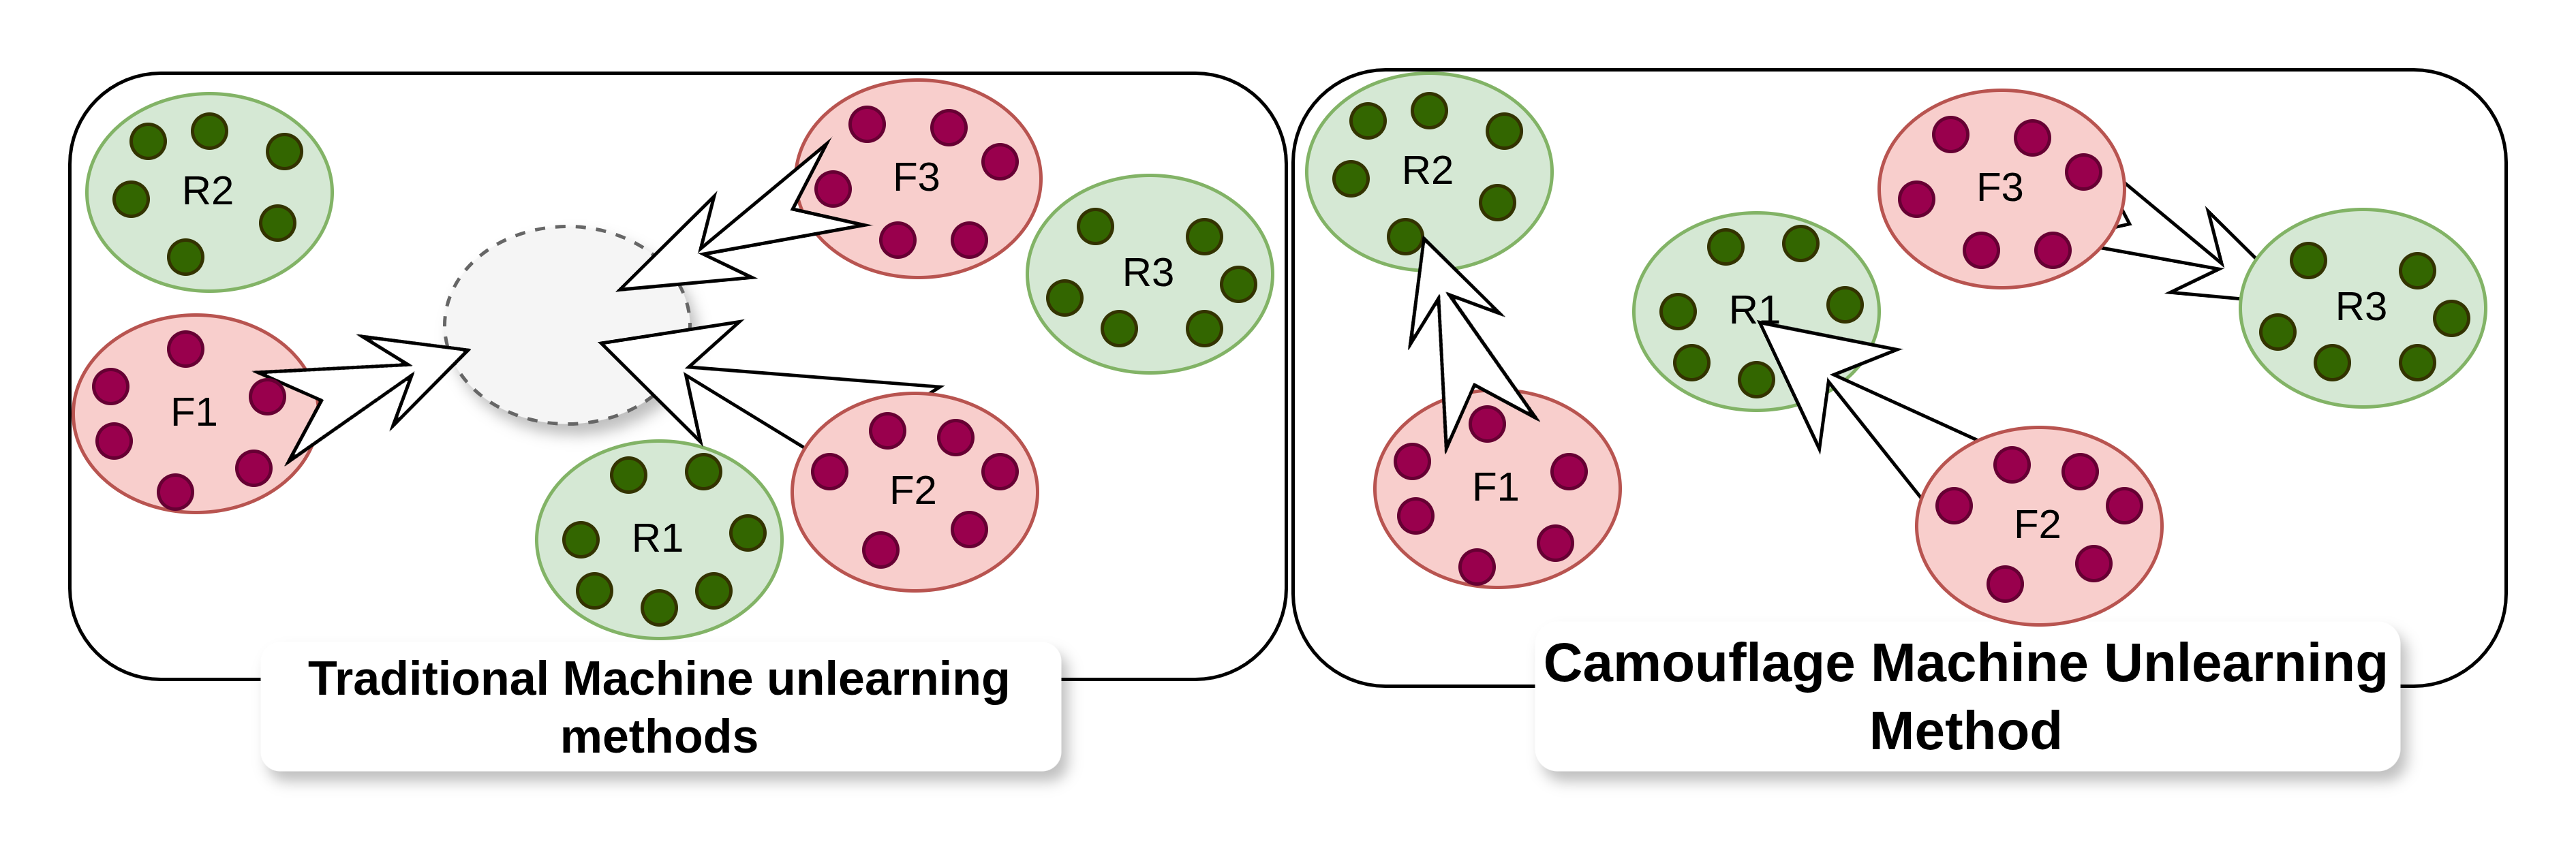
\includegraphics[width=1\textwidth]{images/Cam-Page-5.drawio.png}
    \caption{Overview of Camouflage Unlearning. Traditional methods collapse all forget classes to a single distant point, requiring long migration paths. CU instead hides each forget class within its nearest retain class boundary, reducing migration distance and accelerating convergence.}
    \label{fig:method}
\end{figure*}

\section{Problem Setting}
Let $\mathcal{M}$ be a model pre-trained on dataset $D$, representing a mapping $f_\mathcal{M} : \mathcal{X}_D \rightarrow \mathcal{Y}_D$ from input space $\mathcal{X}_D$ to output space $\mathcal{Y}_D$. Our objective is to selectively discard certain knowledge while preserving remaining knowledge. We partition the data as $D = D_\textit{r}^{\textit{full}} \cup D_\textit{f}$, where $D_\textit{f}$ denotes forget samples and $D_\textit{r}^{\textit{full}}$ denotes retain samples ($D_\textit{r}^{\textit{full}} \cap D_\textit{f} = \emptyset$).

In practice, storing the full retain set is prohibited under GDPR and CCPA regulations for privacy-sensitive data, while for non-private data, retraining remains computationally expensive due to large scale models and datasets. We therefore maintain a small replay buffer $D_\textit{r} \subset D_\textit{r}^{\textit{full}}$ such that $|D_\textit{r}| \ll |D_\textit{r}^{\textit{full}}|$, with $|D_\textit{r}|$ limited to at most 10\% of $|D_\textit{r}^{\textit{full}}|$\footnote{From this point, $D_\textit{r}$ denotes the replay buffer unless specified.}. Before unlearning, $\mathcal{M}$ performs well on $D_\textit{r}$ and $D_\textit{f}$, i.e.,
{\small
\begin{equation}
f_{\mathcal{M}} :
\mathcal{X}_{D_\textit{f}} \rightarrow \mathcal{Y}_{D_\textit{f}} \; ; \;
\mathcal{X}_{D_\textit{r}} \rightarrow \mathcal{Y}_{D_\textit{r}}
\label{eq:1}
\tag{1}
\end{equation}
}

Let the unlearning algorithm be $\mathcal{F}$ detailed in Section~\ref{sec:4}, which modifies model $\mathcal{M}$ to obtain $\mathcal{M}'$ via $\mathcal{M}' = \mathcal{F}(\mathcal{M}, D_\textit{f}, D_\textit{r})$. The unlearned model $\mathcal{M}'$ holds a new mapping $f_{\mathcal{M}'}$:
{\small
\begin{equation}
f_{\mathcal{M}'} :
\mathcal{X}_{D_\textit{f}} \cancel{\rightarrow} \mathcal{Y}_{D_\textit{f}} \; ; \;
\mathcal{X}_{D_\textit{r}} \rightarrow \mathcal{Y}_{D_\textit{r}}
\label{eq:2} \tag{2}
\end{equation}
}
Here, $\cancel{\rightarrow}$ denotes that the mapping no longer holds, i.e., the knowledge is forgotten, while $\rightarrow$ indicates the mapping persists. We define successful unlearning as 
\begin{itemize}
    \item Forgetting: $\textit{Acc}(\mathcal{M}', D_\textit{f}) \leq \frac{1}{C}, $
    \item Retention: $\textit{Acc}(\mathcal{M}', D_\textit{r}) \approx \textit{Acc}(\textit{Oracle}, D_\textit{r})$
\end{itemize}
where $C$ is the number of classes and Oracle denotes a model trained directly on target classes only.